\chapter{Introduction}
\label{chap:intro}

The advancement of gaming device technology such as Kinect, Wii Balance Board, Wii Remote, PlayStation Move, etc. has enabled players to control and interact with the game console through body movement. In healthcare, such technology are used in serious game which can help the users (doctors, patients, researchers, etc.)  perform health related activity such as patients' rehabilitation and training\cite{rahman,brezinka,green}. One example of such game is Hammer and Planks which was designed to train the equilibrium of patient with balance disorders (specifically for hemiplegic people)\cite{diloreto}. A person with hemiplegic is paralized on one side of the body\footnote{\url{http://www.hemihelp.org.uk/hemiplegia/what_is_hemiplegia}}. Therefore, the gameplay is designed so that the player has to move their body to right, left, front and back in order to train their affected side of the body. To support the purpose of rehabilitation, the healthcare professionals need to analyse the movement to  make a correct diagnostic of patients' progress and to adjust the difficulty level for the next rehabilitation session. In this thesis, I discuss the design of an interface to help healthcare professional to understand the data generated from the game.

\section{Motivation}

Hammer and Planks is a vertical shooter game. The game world is in a 2D environment vertically scrolling from top to bottom in which a player navigate a ship from left to right through moving his body(figure \ref{game_screenshot}). It tells the story of a pirate named John K. One day a meteor fell down on John's ship and ruin it. There is a little left from his boat but it is still enough to build a new basic boat with what's left. While navigating his ship to collect driftwood/plank to upgrade it (hence the name Hammer and Planks), he also wants to find the ship which showered meteor and destroyed his ship. Therefore, in the game a player has to defeat all enemies which come on his way and he has to avoid being destroyed by bullets, reefs and other obstacles. Throughout the game the player has to collect bonuses (planks) to improve the ship. The game is usually played in short and intense phase and thus requires a lot of concentration\cite{diloreto}.

Currently, the game provides some charts which visualize player's body movement with respect to the horizontal axis and vertical axis. However, the information that can be gathered from the visualization is not enough for the healthcare professional to be able to establish an informed diagnostic. It's hard to know how often the player move to right or left. It's also not possible to know to which type of events (ie. avoiding an enemy, catching the bonuses) the movement is related to. Which is crucial since the therapist need to know if the player is able to develop strategy to play the game overtime. The existing visualization also provides chart to show the evolution of player's performance and total movement for all game sessions. However, the evolution of player's body movement (horizontally or vertically) is not depicted.

The purpose of this thesis is to address the problem mentioned by proposing three types of visualization:(i)a visualization which provides information related to a certain type of event in the game and body movement for each one game session (ii)a visualization which represents a certain type of event, body movement, and the speed in which the event is occurring in one game session, and (iii)a visualization where healthcare professionals can analyze the evolution of player's body movement throughout all sessions. For the third visualization, there are two options in which the user can analyze the movement: by area of movement or by the number of movement in an area.

\begin{figure}
\centering
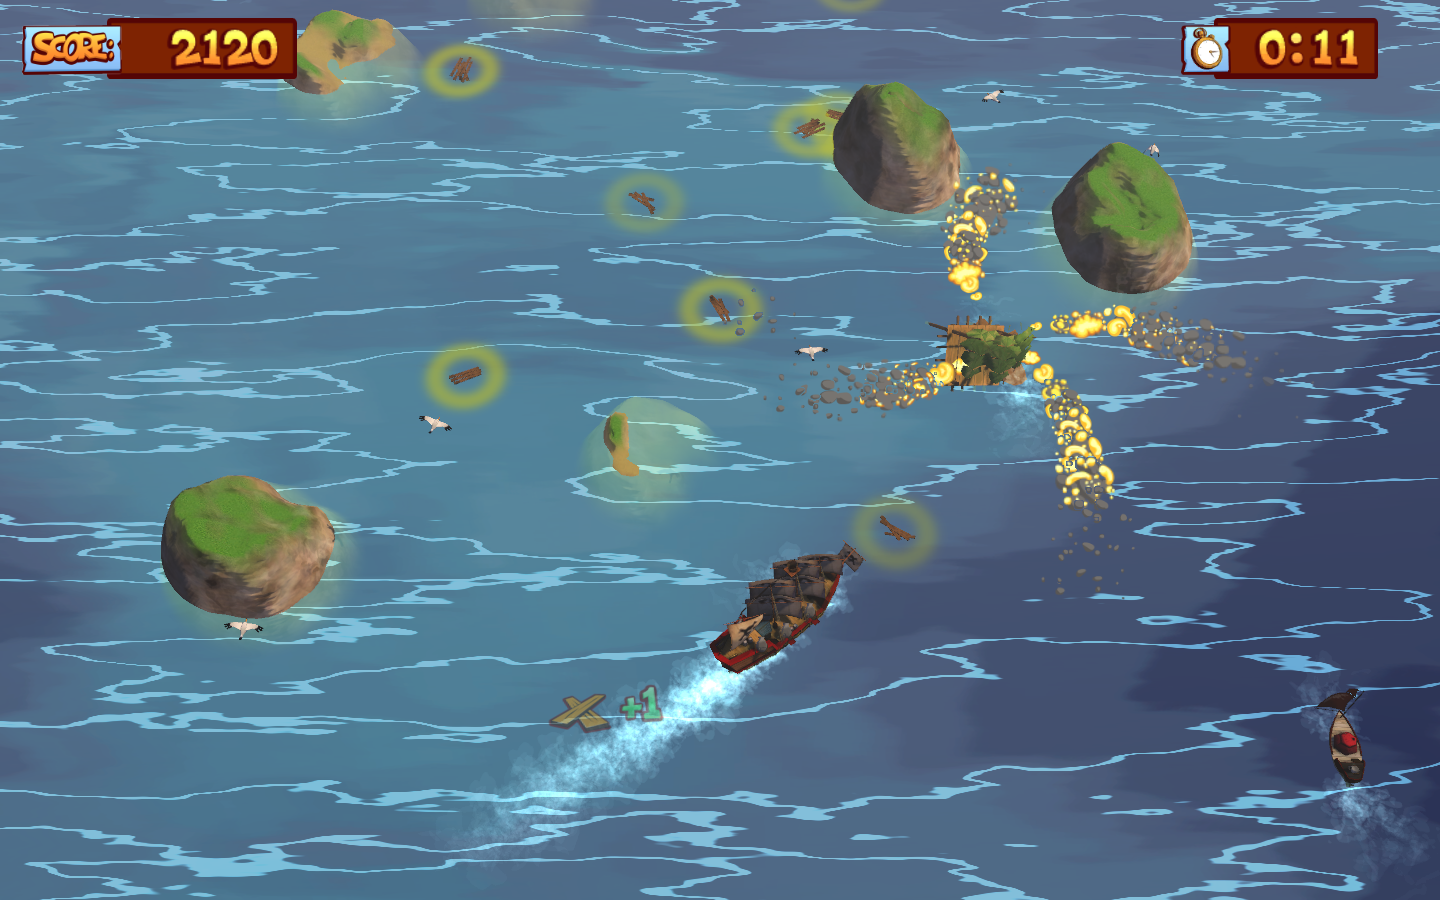
\includegraphics[width=110mm]{hp_game.png}
\caption{Hammer and Planks Screenshot \label{game_screenshot}}
\end{figure}


\section{Methodology}

To ensure that the visualization to be designed would satisfy the information needed by healthcare professionals, I followed the Nested Process Model proposed by Tamara Munzner \cite{Munzner:2009:NMV:1638611.1639181}. The model is divided into 4 levels: Domain Problem Characterization, Data/Operation Abstraction Design, Encoding/Interaction Technique Design, and Algorithm Design. These levels are nested; the output of a higher level will be the input for the lower level as shown in figure \ref{munzner_model}.

\begin{figure}
\centering
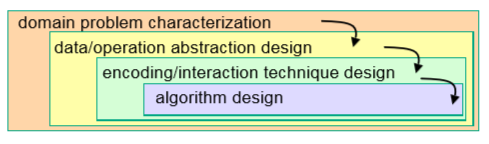
\includegraphics[width=100mm]{munzner_model.png}
\caption{Munzner's Visualization Design Model with four nested layers \label{munzner_model}}
\end{figure}

In domain problem characterization level, I discuss what kind of information needed by health professional from the visualization. The output of this level would be a list of tasks that need to be solved by the visualization application. I then identifies the data structure which can support these tasks in the Data/Operation Abstraction Design level. In the third level, a good visualization and interaction technique which can support the tasks will be defined. For this thesis, I leave out the algorithm design level since there is no new algorithm proposed.

\section{Thesis Outline}

The remainder of this thesis is organized as follows. Chapter 2 discuss the domain problem characterization. Chapter 3 explores related work. The data abstraction is presented in Chapter 4. The Visual Mapping and Interactive Functionality of the proposed visualization are discussed in details in Chapter 5. Chapter 6 provides some case studies used to evaluate the approach and finally, chapter 7 concludes the thesis.
